\section{Transformaciones Mezclantes y Exactas}

\begin{dfn}[Transformaci�n Mezclante] Si $S$ cumple que
\begin{equation}
\limi_{n\rightarrow\infty}{\mu(A\cap S^{-n}(B))}=\mu(A)\mu(B)\qquad \text{para todo} A,B\in\A
\end{equation}
Siendo $(\X,\A,\R)$ es un espacio de medida probabilidad, y $S:\X\cir$ una transformaci�n que preserva la medida.
\end{dfn}

La definici�n de mezclante puede ser interpretada de la siguiente forma.  Los puntos que partieron en A y finalizar�n en B despu�s de n iteraciones su medida est� determinada por el producto de las medidas de A y de B. Adicionalmente, es independiente de la posici�n inicial de $A$ y de $B$ en $\X$.

\subparagraph{Observaci�n} Es f�cil de ver cualquier transformaci�n de mezclante esta deber� ser erg�dica. Se asume que
$B\in\A$ es un conjunto invariante, en que se cumple $B=S^{-1}(B)$ y,  a�n m�s, $B=S^{-n}(B)$  por inducci�n. Se toma $A=\X  $
para que $\mu(A\cap B)=\mu(A\cap S^{-b}(B))=0$. Sin embargo, de que debe tener
y por lo tanto es o bien 0 o 1, lo que demuestra la ergodicidad

\begin{dfn}[Transformaci�n Exactas] Si $S$ cumple que
\begin{equation}
\limi_{n\rightarrow\infty}{\mu(S^n(A))}=1 \qquad \hbox{para cada $A\in\A, \mu(A)>0$}  
\end{equation}
Siendo $(\X,\A,\R)$ es un espacio de medida probabilidad, y $S:\X\cir$ una transformaci�n que preserva la medida.
\end{dfn}

Para ejemplificar la diferencia entre los tipos de transformaci�n se procede a mostra las seis primeras iteraciones de un 
n�mero aleatorio de 1000 puntos distribuidos en el conjunto de $\X=[0,1]\times[0,1]$ 

{\bf Transformaci�n Erg�dica}
\begin{equation}
S(x,y)=(\sqrt{2}+x,\sqrt{3}+y)\quad (mod\; 1)\label{t.erg}
\end{equation}
{\bf Transformaci�n Mezclante}
\begin{equation}
S(x,y)=(x+y,x+2y)\quad (mod \;1)\label{t.mez}
\end{equation}
{\bf Transformaci�n Exacta}
\begin{equation}
S(x,y)=(3x+y,x+3y)\quad (mod \;1)\label{t.exa}
\end{equation}


\begin{figure}
    \begin{center}
        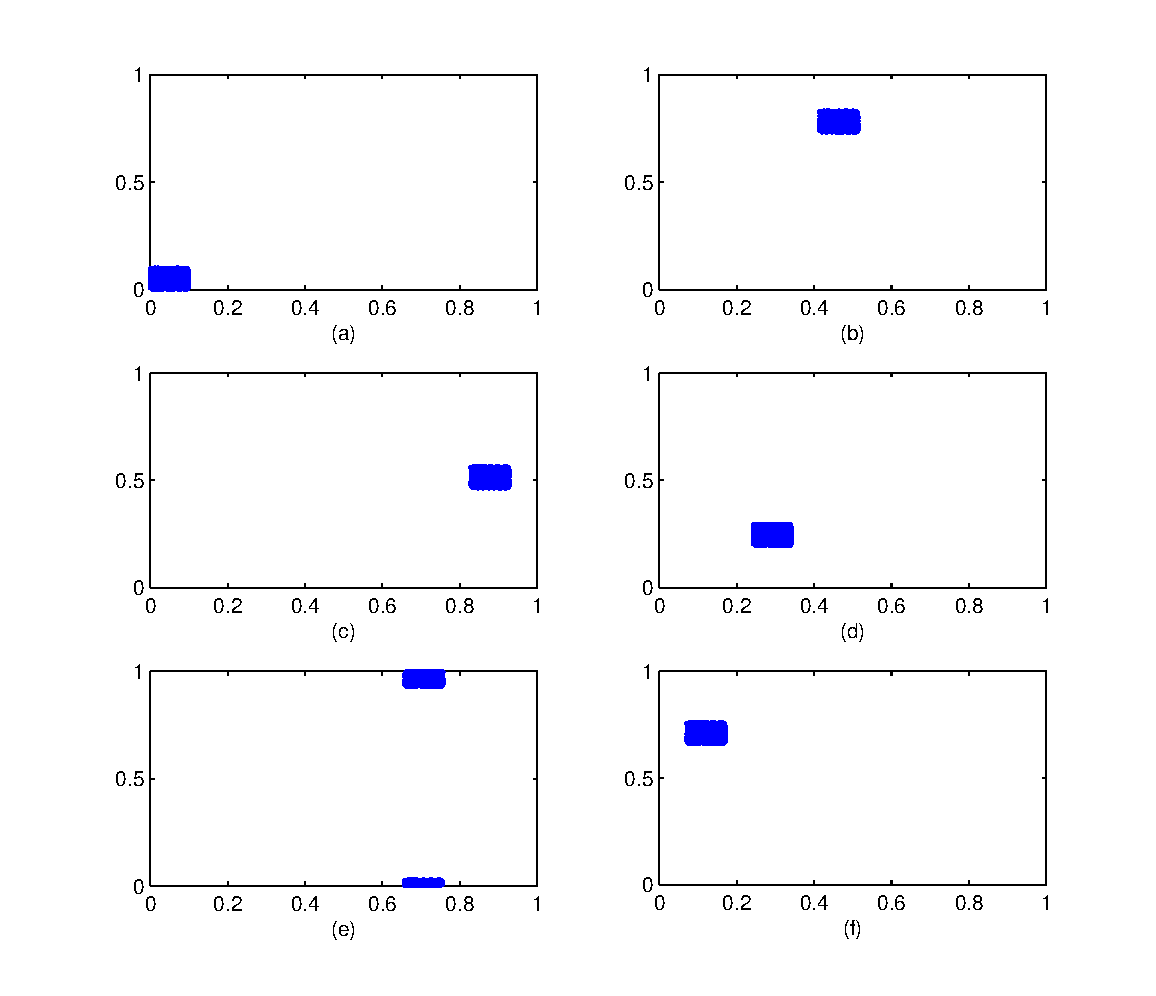
\includegraphics[width=.65\textwidth, height=1\textwidth,scale=0.5]{graficas/erg}
    \end{center}
    \caption{Iteraciones sucesivas de la transformaci�n \ref{t.erg}. Note como se mueve la distribuci�n de puntos en forma de cudrado sobre el espacio}

\end{figure}

\begin{figure}
    \begin{center}
        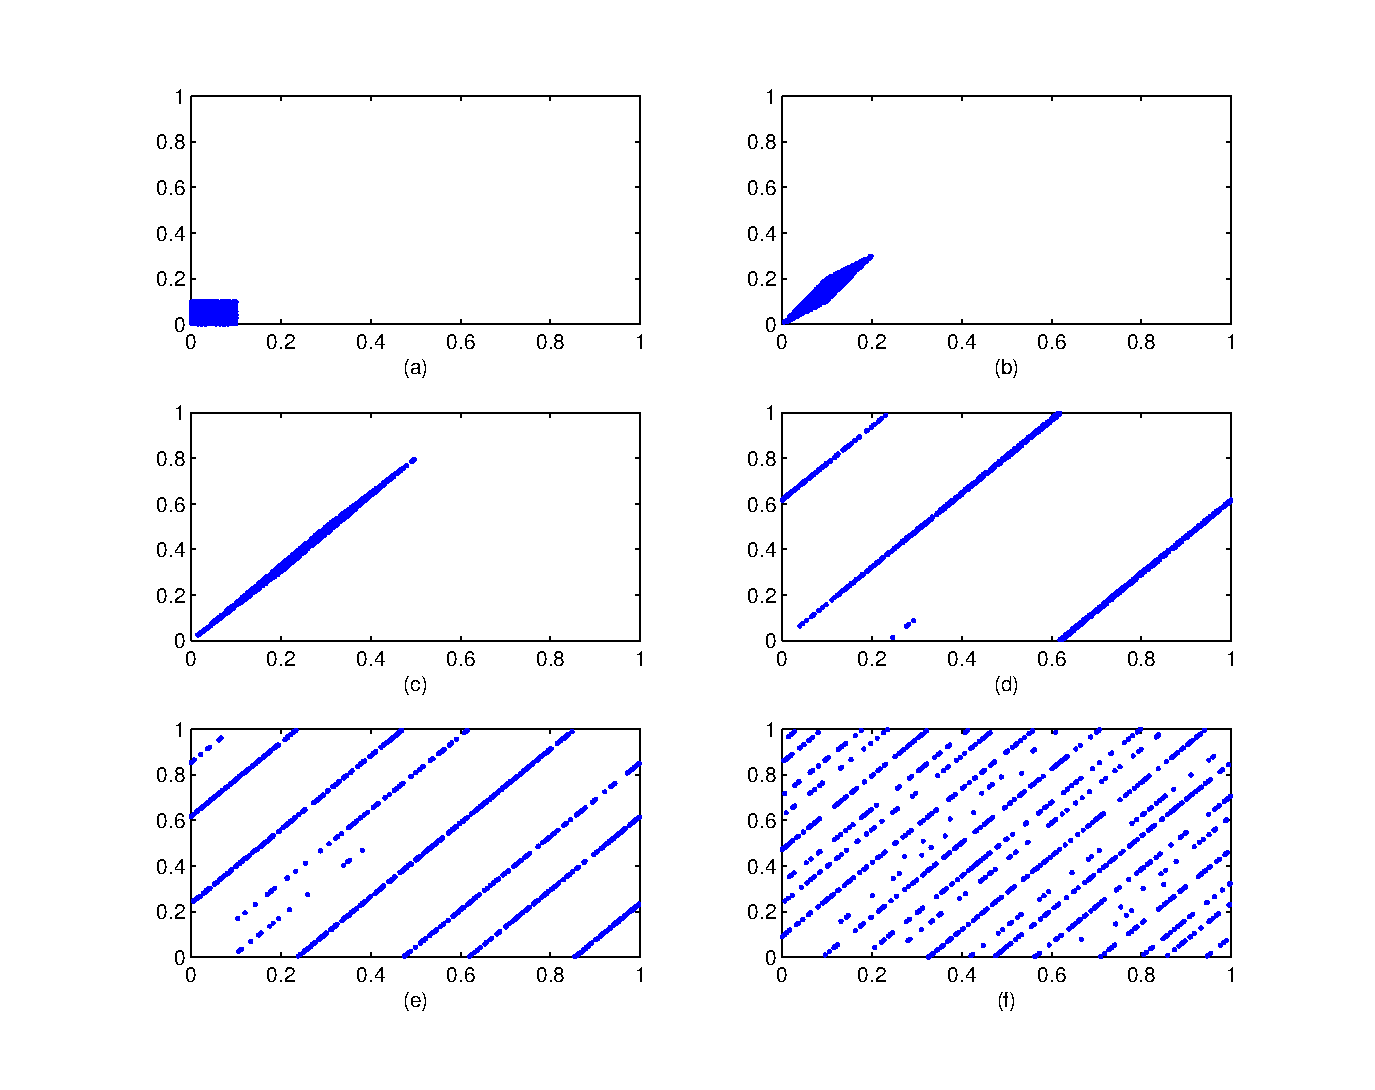
\includegraphics[width=.65\textwidth, height=1\textwidth,scale=0.5]{graficas/mix}
    \end{center}
    \caption{Iteraciones sucesivas de la transformaci�n \ref{t.mez}. Note como se esparce la distribuci�n de puntos sobre el espacio}

\end{figure}


\begin{figure}
    \begin{center}
        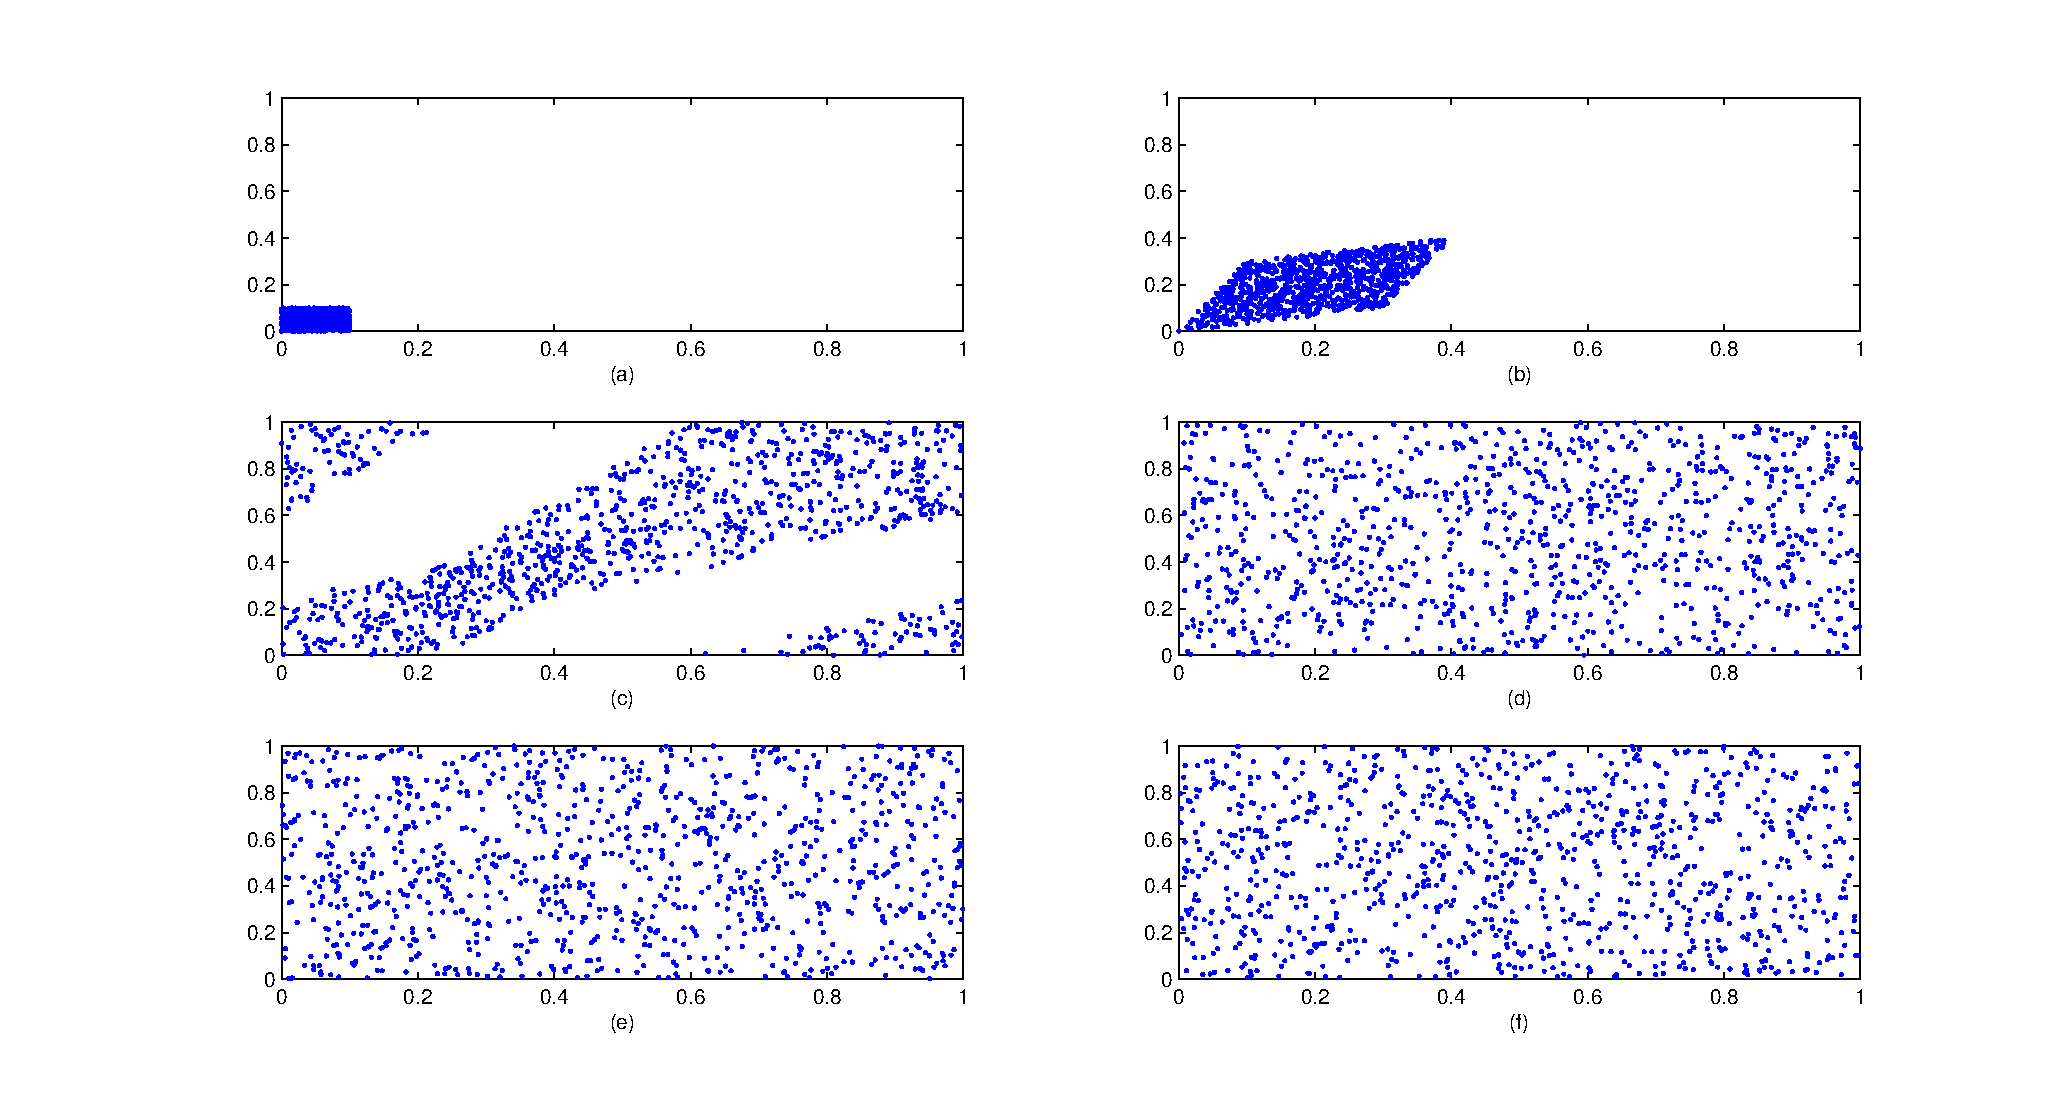
\includegraphics[width=.65\textwidth, height=1\textwidth,scale=0.5]{graficas/exa}
   \end{center}
    \caption{Iteraciones sucesivas de la transformaci�n \ref{t.exa}. Note como se esparce la distribuci�n de puntos sobre el espacio}

\end{figure}

\section{Taxonom�a de las Transformaciones}

Los conceptos desarrollados en las secciones previas para clasificar varios niveles de irregularidad en el comportamiento
est�n escritos en t�rminos de comportamiento de sucesiones de conjuntos. La pruebas de ergodicidad, mezclante o exacta
usando las definiciones son dif�ciles. En efecto los ejemplos presentados hasta ahora ilustran estos conceptos, no son rigurosas pruebas.

En esta secci�n se reformular� los conceptos de ergodicidad, mezclante y exacta en t�rmino del comportamiento de
sucesiones de iteraciones de los operadores de Perron-Forbenius y Koopman. Para mostrar c�mo pueden ser usadas para
determinar si una transformaci�n $S$ junto con una medida invariante es erg�dica, mezclante o exacta. Se requerir�
nociones sobre convergencia Cesaro, D�bil y Fuerte.

\begin{teo}Sea $(\X,\A,\R)$ una espacio de medida, $S:\X\cir$ una medida que preserva la transformaci�n y P el
    operador de Perron-Frobenius correspondiente a S. Entonces:
    \begin{description}
        \item[La transfomaci�n $S$ es erg�dica] si y solo si la sucesi�n converge Cesaro a 1 para todo $f\in D$.
        \item[La transfomaci�n $S$ es mezclante] si y solo si la sucesi�n converge d�bilmente a 1 para todo $f\in D$.
        \item[La transfomaci�n $S$  es exacto] si y solo si la sucesi�n converge fuertemente  a 1 para todo $f\in D$.
    \end{description}
\end{teo}

\subparagraph{Observaci�n} Note que como el operador $\Pm$ es lineal, la convergencia de la sucesi�n $\{\Pm^n f\}$ a 1 para
    $f\in D$ es equivalente a la convergencia de $\{\Pm^n f\}$ a $<f,1>$ para cada $f\in L^1$. Esta observaci�n es
    validad para todos los tipos de convergencia: Cesaro, D�bil, Fuerte. Por lo tanto,se reescribe el teorema.

\begin{teo}Sea $(\X,\A,\R)$ una espacio de medida, $S:\X\cir$ una medida que preserva la transformaci�n y $\Pm$
    el operador de Perron-Frobenius correspondiente a S. Entonces:
    \begin{description}
        \item[La transfomaci�n $S$ es erg�dica] si y solo si
        $$\limi_{n\rightarrow\infty}{\frac{1}{n}\sum_{k=0}^{n-1}{<\Pm^k f,g>=<f,1><1,g>}}\qquad f\in L^1,g\in L^\infty$$
        \item[La transfomaci�n $S$ es mezclante] si y solo si
        $$\limi_{n\rightarrow\infty}{<\Pm^k f,g>=<f,1><1,g>}\qquad f\in L^1,g\in L^\infty$$
        \item[La transfomaci�n $S$  es exacto] si y solo si
        $$\limi_{n\rightarrow\infty}{||\Pm^k f -<f,1>||>=0}\qquad f\in L^1$$
    \end{description}
\end{teo}

\begin{proof} Se probar� unicamente la condici�n de mezclante. Se asume la condici�n de
transformaci�n $S$ mezclante entonces por definici�n
\begin{align*}
    \limi_{n\rightarrow\infty}\mu(A\cap S^{B})&=\mu(A)\mu(B)  \\
\intertext{Reescribiendola en su forma integral}
    \limi_{n\rightarrow\infty}\int_\X\car_A(x)\car_B(x)(S^n(x))\mu(dx)&=\int_X\car_A(x)\mu(dx)\int_X\car_B(x)\mu(dx)\\
\intertext{Aplicando la definici�n del operador de Koopman}
    \limi_{n\rightarrow\infty}\int_\X\car_A(x)U^n\car_B(x)\mu(dx)&=\int_X\car_A(x)\mu(dx)\int_X\car_B(x)\mu(dx)\\
\intertext{Aplicando la defunci�n de producto escalar}
    \limi_{n\rightarrow\infty}<\car_A,U^n\car_B>&=<\car_A,1><1,\car_B>\\
\intertext{Usando la propiedad \eqref{c2n3} el operador de Perron-Frobenius es adjunto del operador de Koopman}
    \limi_{n\rightarrow\infty}<\Pm^n \car_A,\car_B>&=<\car_A,1><1,\car_B>\\
\intertext{Con lo que queda demostrado para $f=\car_A$ y $g=\car_B$.}
\end{align*}

Supongamos que $\tilde{A}=\cup_{i=1}^n{A_i}$, $\tilde{B}=\cup_{j=1}^m{B_j}$ y $\nu(A_i)=\lambda_k\delta_{ki}\mu(A_i)$
donde $\delta_{ik}$ es la delta de kronecker. N�tese que $\nu$ define una medida; supongase que S es mezclante, en consecuencia.

\begin{align*}
    \limi_{n\rightarrow\infty}\nu(\tilde{A}\cap S^{-1}(\tilde{B}))
     &=\limi_{n\rightarrow\infty}\nu(\cup_{i=1}^l{A_i}\cap S^{-1}(\cup_{j=1}^m{B_j})) \\
\intertext{Sustituyendo la definici�n de $\nu$}
     &=\limi_{n\rightarrow\infty}\lambda_h\delta_{hi}\lambda_k\delta_{kj}\sum_{i=1}^l{\sum_{j=1}^m{\mu(A_i\cap S^{-1}(B_j))}} \\
\intertext{Propiedades de la medida}
     &=\limi_{n\rightarrow\infty}\sum_{i=1}^l{\sum_{j=1}^m{\lambda_h\delta_{hi}\lambda_k\delta_{kj}\mu(A_i\cap S{-1}(B_j))}}\\
\intertext{Por linealidad}
     &=\limi_{n\rightarrow\infty}\sum_{i=1}^l{\sum_{j=1}^m{\lambda_i\lambda_j\mu(A_i\cap S{-1}(B_j))}} \\
\intertext{Evaluando las deltas de kronecker}
     &=\limi_{n\rightarrow\infty}\sum_{i=1}^l{\sum_{j=1}^m{\lambda_i\lambda_j\int_X{\car_{A_i}(x)\car_{B_j}(x)(S^n(x))\mu(dx)}}}\\
     &=\limi_{n\rightarrow\infty}\int_\X{\sum_{i=1}^l{\car_{A_i}(x)}\sum_{j=1}^m{U^n \car_{B_j}(x)\mu(dx)}}\\
     &=\limi_{n\rightarrow\infty}<\sum_{i=1}^l{\lambda_i\car_{A_i}(x)},\sum_{j=1}^m{U^n\lambda_j \car_{B_j}(x)}>\\
     &=\limi_{n\rightarrow\infty}<\sum_{i=1}^l{\Pm^n\lambda_i\car_{A_i}(x)},\sum_{j=1}^m{\lambda_j\car_{B_j}(x)}>\\
\intertext{Por otro lado, como $\nu$ es mezclante se tiene}
 \nu(A)\nu(B)&=\nu(\cup_{i=1}^l{A_i})\nu(\cup_{j=1}^m{B_j})  \\
             &=\lambda_h\delta_{hi}\sum_{i=1}^l{\mu(A_i)}\lambda_k\delta_{kj}\sum_{j=1}^m{\mu(B_j)}\\
             &=\sum_{i=1}^l{\lambda_i\mu(A_i)}\sum_{j=1}^m{\lambda_j\mu(B_j)}\\
             &=\sum_{i=1}^l{\lambda_i\int_\X\car_A(x)\mu(dx)}\sum_{j=1}^m{\lambda_j\int_X{\car_B(x)\mu(dx)}}\\
             &=\int_\X{\sum_{i=1}^l{\lambda_i\car_A(x)\mu(dx)}}\int_\X{\sum_{j=1}^m{\lambda_j\car_B(x)\mu(dx)}}\\
             &=<\sum_{i=1}^l{\lambda_i\car_{A_i}},1><1,\sum_{j=1}^m{\lambda_j\car_{B_i}}>
\end{align*}
Y por lo tanto se cumple para funciones simples. Adicionalmente, para cada $g\in L\infty$ es convergente a un limite de funciones simples en 
$g_k\in\infty$ y para cada funci�n $f\in L^1$ tiene convergencia fuertemente a la sucesi�n de funciones simples $f_h\in L^1$. Se tiene la siguiente relaci�n
\begin{align*}
|<\Pm^n f, g>-<f,1><1,g>|&\leq|<\Pm f,g>-<\Pm^n f_k,g_k>|\\
                         &+|<\Pm^n f_k,g_k>-<f_k,1><1,g_k>|\\
                         &+|<f_k,1><1,g_k>-<f,1><1,g>|   
\end{align*}  

Si $||f_k-f||\leq\epsilon$ y $||g_k-g||\leq\epsilon$ entonces se satisface 
\begin{align*}
|<\Pm f,g>-<\Pm^n f_k,g_k>|&\leq|<\Pm^n f,g>-<\Pm^n f_k,g>|\\
                           &+|<\Pm^n f_k,g>-<\Pm^n f_k,g_k>|\\
                           &\leq\epsilon ||g||_{L^\infty}+\epsilon||f_k||\\
                           &\leq\epsilon(||g||_{L^\infty}+||f||+\epsilon)
\end{align*}

Se forma analoga se prueba 

$$|<f_k,1><1,g_k>-<f,1><1,g>|\leq\epsilon(||g||_{L\infty}+||f||+\epsilon)$$

Como estos t�rminos son arbitrariamente peque�os para $\epsilon$. Finalmente, el t�rmino

$$|<\Pm^n f_k,g_k>-<f_k,1><1,g_k>|$$ 

Converge a cero para $n\rightarrow\infty$. Esto completa la prueba de que es mezclante implica $<\Pm^n f,g>$ a $<f,1><1,g>$ para todo 
$f\in L^1$ y $g\in L^\infty$. La implicaci�n opuesta se demuestra tomando el conjunto $f=\car_A$ y $g=\car_B$.

\end{proof}


